\documentclass[tikz,border=10pt]{standalone}
\usepackage{tikz}
\usepackage{amsmath}

\begin{document}
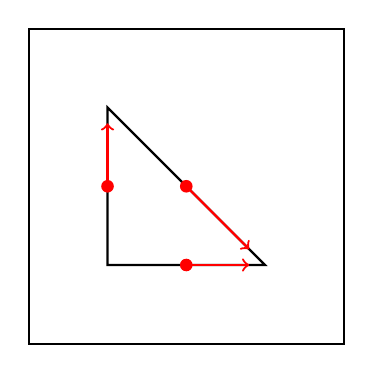
\begin{tikzpicture}[scale=2]
    % Define the vertices of the reference triangle
    \coordinate (A) at (0,0);
    \coordinate (B) at (1,0);
    \coordinate (C) at (0,1);

    \coordinate (N1) at (0.5,0);
    \coordinate (N2) at (0,0.5);
    \coordinate (N3) at (0.5,0.5);

    \coordinate (G0) at (-0.5,-0.5);  
    \coordinate (G1) at (-0.5,1.5);  
    \coordinate (G2) at (1.5,1.5);  
    \coordinate (G3) at (1.5,-0.5);  
    \draw[black, thick] (G0) -- (G1) -- (G2) -- (G3) -- cycle;




    % Draw the triangle
    \draw[black, thick] (A) -- (B) -- (C) -- cycle;

    % Label the vertices
%    \node[below left] at (A) {$A$};
%    \node[below right] at (B) {$B$};
%    \node[above left] at (C) {$C$};

    % Draw vector fields with arrows
	\draw[->, red, thick] (0.5, 0) -- (0.9, 0.0);   
	\draw[->, red, thick] (0.5, 0.5) -- (0.9,0.1);   
	\draw[->, red, thick] (0, 0.5) -- (0.0, 0.9);  

    % Local coordinate system within the triangle
%    \node at (1.5,1) {$\mathbf{u}(x,y) = \begin{pmatrix} a + bx \\ c + dy \end{pmatrix}$};

    \fill[red] (N1) circle (0.04);
    \fill[red] (N2) circle (0.04);
    \fill[red] (N3) circle (0.04);


\end{tikzpicture}
\end{document}



